\documentclass{article}
\usepackage[utf8]{inputenc}
\parskip = 0.75em
\parindent = 10mm
\def\baselinestretch{1}
\usepackage {float}
\usepackage{listings}
\usepackage{subcaption}
\usepackage[usenames]{color}
\usepackage[numbers,sort&compress]{natbib}
\usepackage{multirow, array}
\usepackage[spanish]{babel}
	\deactivatetilden
	\spanishdecimal{.}
	\addto\captionsspanish{\def\tablename{Tabla}}
	\addto\captionsspanish{\def\listtablename{\'Indice de tablas}}

\usepackage{amsmath,amsfonts,amssymb}
	\allowdisplaybreaks[4]
\usepackage{graphicx}
	\graphicspath{{Figuras/}}
\usepackage[clearempty,pagestyles]{titlesec}
\usepackage{anysize}

\def\baselinestretch{1.5}
\papersize{27.9cm}{21.5cm} 
\marginsize{2cm}{2cm}{1cm}{1cm}

\begin{document}


	\begin{center}
	\huge{\textbf{Tarea 12 Red neuronal}}\\
	
	\textsc{ \Large Susana Ruiz Nuñez}
	\end{center}


\section{Planteamiento del problema} 
En esta práctica \cite{satu} se estudia una demostración básica de aprendizaje a máquina.  A reconocer dígitos de imágenes pequeñas en blanco y negro con una red neuronal. Se tienen los elementos básicos de una red neuronal; el perceptrón que esencialmente es un hiperplano que busca ubicarse en la frontera que separa las entradas verdaderas de las falsas. La dimensión  del perceptrón es el largo del vector  que toma como entrada, y su estado interno se representa con otro vector que contiene sus pesos. Para responder a una salida proporcionada a ello, el perceptrón calcula el producto interno y si esta suma es positiva, la salida del perceptrón es verdad, en otro caso es falso.

\section{Metodología}
Para el desarrollo de la tarea se generan una serie de dígitos y se requiere analizar el desempeño de la red neuronal en términos de puntaje F (F-- score) en función de las probabilidades asignadas a la generación de los dígitos \cite{metr}. El puntaje F consiste en un test de medida de precisión que se suele hacer para probar algoritmos. Se considera una media armónica que combina los valores de la precisión y exhaustividad de la siguiente manera:

\begin{equation}
	Fscore= 2 * \frac{Precision * Exhaustividad}{Precision + Exhaustividad} 
\end{equation}

\section{Experimentación}

Se analizan tres ' Estados de Probabilidad ' del modelo donde se varía la probabilidad en cada uno de ellos de la generación de dígitos de la siguiente manera,  (n: negro, g: gris, b: blanco): 

\begin{itemize}
	\item El estado 1 al que se le denomina 'Probabilidad1': n = 0.995, g = 0.92, b = 0.002
	\item El estado 2 al que se le denomina 'Probabilidad2': n = 0.902, g = 0.99, b = 0.005
	\item El estado 3 al que se le denomina 'Probabilidad3': n = 0.605, g = 0.82, b = 0.992
\end{itemize}

El estado 1 consiste en el estado inicial del problema, se mantuvieron las probabilidades sin realizarle ningún cambio. Se muestra en el análisis de puntaje F, como tiene altos niveles de precisión a la hora de determinar el dígito correcto, sus valores se encuentran entre los 0.5 y 0.9, con un promedio de 0.857. Se observa más exactitud en algunos dígitos que en otros.   
\begin{lstlisting}[language=Python]
			precision    recall  f1-score   support
			
			0      0.700     0.412     0.519        34
			1      1.000     0.918     0.957        49
			2      1.000     1.000     1.000        35
			3      0.971     0.944     0.958        36
			4      1.000     0.739     0.850        23
			5      1.000     1.000     1.000        26
			6      0.731     1.000     0.844        19
			7      0.950     0.950     0.950        20
			8      0.406     0.591     0.481        22
			9      0.784     1.000     0.879        29
			
		accuracy                           0.857       293
		macro avg      0.854     0.855     0.844       293
		weighted avg   0.875     0.857     0.856       293
\end{lstlisting}

Para el estado 2 se hizo una variación conservadora de las probabilidades, se disminuyó ligeramente la del color negro y para los colores restantes se aumentaron los valores. Con esta variación la precisión se mantuvo constante para casi todos los dígitos, el puntaje F si disminuyó con un promedio de 0.733.  
\begin{lstlisting}[language=Python]
			precision    recall  f1-score   support

			0      0.929     0.722     0.813        36
			1      0.914     0.727     0.810        44
			2      0.824     0.800     0.812        35
			3      0.650     0.650     0.650        20
			4      0.800     0.683     0.737        41
			5      0.519     0.519     0.519        27
			6      0.722     0.812     0.765        16
			7      0.718     0.824     0.767        34
			8      0.625     0.833     0.714        18
			9      0.480     0.857     0.615        14

		accuracy                          0.733       285
		macro avg     0.718     0.743     0.720       285
		weighted avg  0.759     0.733     0.738       285
\end{lstlisting}

Para el estado 3 si se hizo una variación considerable, con la finalidad de ver que ocurría si se cambiaban por completo los valores. Se aumentó como probabilidad máxima el del blanco y se hicieron grandes variaciones para los otros dos colores. Por consiguiente el comportamiento del puntaje F disminuyó hasta un 0.265, dando como resultado que hubieran dígitos que no los reconociera ni una sola vez.

\begin{lstlisting}[language=Python]
			precision    recall  f1-score   support
	
			0      0.150     0.083     0.107        36
			1      0.739     0.386     0.507        44
			2      0.379     0.314     0.344        35
			3      0.125     0.200     0.154        20
			4      0.333     0.268     0.297        41
			5      0.250     0.407     0.310        27
			6      0.062     0.062     0.062        16
			7      0.318     0.538     0.400        13
			8      0.000     0.000     0.000         3
			9      0.100     0.071     0.083        14
	
		accuracy                       	   0.265       249
		macro avg      0.246     0.233     0.227       249
		weighted av    0.324     0.265     0.278       249
\end{lstlisting}


\section{Resultados}

Los resultados que muestra la gráfica tienen estrecha relación con lo presentado hasta ahora. Se muestra como el desempeño de la red neuronal va variando según se cambian las probabilidades asignadas a la generación de dígitos. En este caso en particular, disminuyó la precisión cada vez que se disminuía la probabilidad con que se genera el color negro y se aumentaba la del color blanco. Los mejores resultados obtenidos para esta experimentación fueron dados con las probablidades iniciales.  


\begin{figure}[H]
\centering
	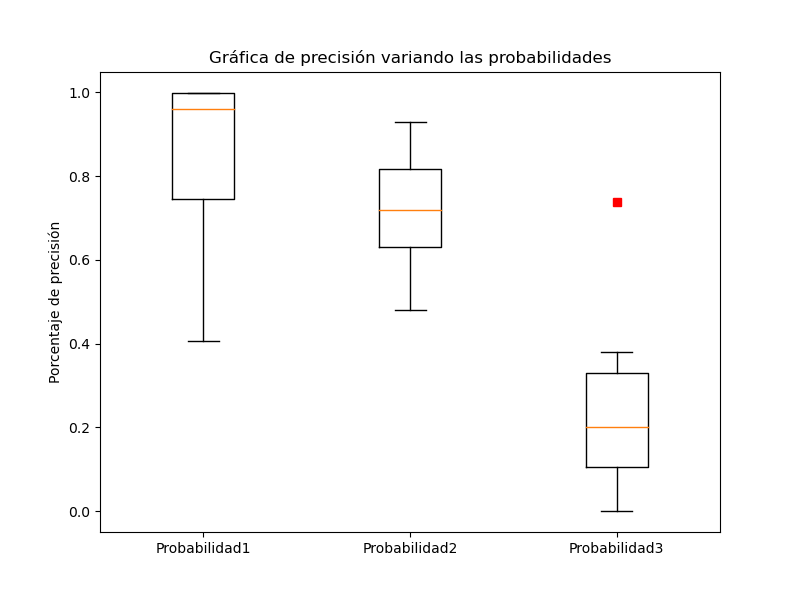
\includegraphics[scale=0.8]{Figure_1.png}
	\caption{Desempeño de la red neuronal con variación en las probabilidades de generación de dígitos.}
	\label{1}		
\end{figure}



\section{Conclusiones}
Se concluye con los experimentos realizados que a la hora de aplicar algoritmos de red neuronal es necesario hacer un análisis previo de los mejores valores a asignar para la generación de la variable para la que se esté desarrollando el proyecto en cuestión.

\bibliography{Tarea12}
\bibliographystyle{plainnat}
\end{document} 
